%\documentclass{emulateapj}
\documentclass[letterpaper,12pt,preprint]{aastex}

% packages
\usepackage{amssymb,amsmath,amsbsy}
\usepackage{booktabs}

% commands
\newcommand{\given}{\,|\,}
\newcommand{\dd}{\mathrm{d}}
\newcommand{\transpose}[1]{{#1}^{\mathsf{T}}}
\newcommand{\inverse}[1]{{#1}^{-1}}
\newcommand{\Msun}{\mathrm{M}_\odot}
\newcommand{\bs}[1]{\boldsymbol{#1}}

\begin{document}

\title{The Companion Mass Distribution to the ELM WD Sample}
\author{Jeff Andrews\altaffilmark{\colum}, Adrian M. Price-Whelan\altaffilmark{\colum}, Marcel Ag\"ueros\altaffilmark{\colum}}

% Affiliations
\newcommand{\colum}{1}
\altaffiltext{\colum}{Department of Astronomy, 
		              Columbia University, 
		              550 W 120th St., 
		              New York, NY 10027, USA}


\begin{abstract}
Determining component masses of single-line spectroscopic binary stars
is impossible because of the unknown inclination angle. Even when the
mass of the bright star can be derived, only a lower limit can be placed
on the mass of the unseen companion. However, since the probability of
any inclination angle scales with sin $i$, for a large enough, unbiased
population, the companion mass distribution can be deconvolved from the
inclination angle. We develop a Bayesian technique to handle this
deconvolution and place it within a Markov Chain Monte Carlo framework.
We then apply our method to the sample of 55 extremely low mass (ELM)
WDs with radial velocity variations. Modeling the companion mass
distribution as a Gaussian with a variable neutron star component, we
find the companion population is well modeled by a mean of 0.65 and a
standard deviation of 0.3 . Our model indicates a neutron star (NS)
fraction of 1.4$\substack{+7.0 \\ -1.4}$\%.
\end{abstract}


\section{Introduction}

The dramatic increase in the number of spectroscopically confirmed white dwarfs (WDs) is seen in the most recently compiled sample from the Data Release 7 (DR7) in the Sloan Digital Sky Survey (SDSS), containing some 20,000 confirmed WDs \citet{kleinman13}. While the distribution of WD masses is strongly peaked at $0.6~\Msun$, a small but non-negligible number (6\%) of low mass WDs (LMWD) was observed, with $M<0.4~\Msun$. In addition to SDSS, LMWDs have been observed in similar numbers elsewhere \citep[e.g. the Palomar Green Survey][]{liebert05}.


Except in special cases of extreme metallicity \citep{kilic07}, the Galaxy is not old enough to produce these LMWD through single star evolution. These objects are formed through dynamical interactions with another star, in which the primary overfills its Roche lobe in either an unstable, common envelope \citep{vdSluys06}, or a phase of stable but non-conservative mass transfer \citep{woods12}. After the primary has become a WD, the secondary overfills its Roche lobe, forming a common envelope prior to core helium ignition, leaving a helium core WD secondary in a tight orbit with either a He- or CO- core WD \citep{han98}.

In their seminal work, \citet{marsh95} discovered companions around five LMWDs in their sample of seven objects, cementing LMWDs as fruitful targets for close binary searches. Using a reduced proper motion selection criterion, the Extremely Low Mass (ELM) WD Survey specifically searched for LMWDs in SDSS using a photometric constraint combined with a reduced proper motion constraint. After their initial investigation found 11 of 12 LMWDs had close binary companions \citep{ELMI}, further radial velocity follow-up has now brought the sample of ELM WDs to 61 systems, 55 of which have measured radial velocity variations \citep{ELMII, ELMIII, ELMIV, ELMV}.


While the orbital periods and radial velocities indicated the companions were most likely WDs, it was realized that these LMWDs could have NS companions \citep{vLeeuwen07}. However this and other radio searches for pulsed emission, as well as searches for blackbody X-ray emission using {\it XMM-Newton} and {\it Chandra}, have all been fruitless \citep{agueros09a,agueros09b,kilic13}. Yet, such systems must exist since LMWDs are observed as companions around millisecond pulsars. Since the orbital solutions provided by the ELM survey combined with the precision of radio data would overconstrain the system, finding even one system would be extraordinarily interesting. The NS binaries with WD companions bright enough to detect spectroscopic radial velocity variations have precisely determined NS masses, allowing for an understanding of the binary evolution processes forming these systems \citep{vKerkwijk96,callanan98,bassa06,antoniadis12}. The resources required for these targeted observations, selecting the most likely candidates for multiwavelength follow-up is crucial. We outline the standard technique below.


For each WD in a single-line spectroscopic binary, spectroscopic observations provide the orbital period ($P_{\rm orb}$), WD mass ($M_1$), and projected orbital velocity ($K$). Using Kepler's third law, we can write the relation between these quantities and the unknown inclination angle as:

\begin{equation}
	\frac{M_2^3}{\left(M_1+M_2\right)^2} {\rm sin}^3 i = \frac{P_{\rm orb}}{2\pi G} K^3 = m_f \label{eq:massfunc}
\end{equation}

The righthand side of this equation is the well-known mass function ($M_f$). $M_2$ is minimized for an edge-on orbit, with $i = 90^{\circ}$. For any individual system, deriving the likelihood of a $M_2$ for that system ($P(M_2)$) involves solving Equation 1 for $M_2$ for different values for $i$, weighting the inclination angle by sin $i$. A basic calculation for the probability that the companion to any individual system is a NS can therefore be calculated:

\begin{equation}
P({\rm NS}) = \int_{0^{\circ}}^{i_{\rm NS}} {\rm sin}\ i\ {\rm d}i \label{eq:P_NS_approx}
\end{equation}

Where $i_{\rm NS}$ is the inclination angle from Equation 1 when $M_2$ is the mass of a NS, typically $\approx1.35~\Msun$. However, implicit in this calculation is that all companion masses are equally likely a priori. Clearly this is not the case as evidenced by \citep{kleinman13} who show the WD mass distribution in SDSS is strongly peaked around $0.6~\Msun$. Including this as a prior on the companion mass does not improve the situation since it is unlikely that the mass distribution of single WDs and WDs in binaries is the same. Equation 2 should therefore be used only as an approximation for the NS probability of a companion.


With 55 systems with precise $M_1$, $P_{\rm orb}$, and $K$, the ELM sample is large enough to be statistically modeled. Furthermore, since the population was selected based on characteristics determined by the primary mass alone, at least with regard to the inclination angle and companion mass, the population is unbiased. In this work we develop a model to determine the mass distribution of companions to ELM WDs in an attempt to answer several specific scientific questions: 1.\ Can the population as a whole be modeled using a simple description of the companion masses? 2.\ How many NSs does our simplistic model imply? 3.\ Can we determine the improved likelihood of any individual system having a NS companion, taking into account the overall rate of NS's in the sample implied by our model? 4.\ Are the six systems without detected radial velocity variations consistent with the population as a whole, or are these a fundamentally separate population (i.e. single ELM WDs)? 5.\ Can our model place limits on the space density of ELM WD binaries with NS companions? 


In Section 2 we build the mathematical framework that we employ in our model described in Section 3. Section 4 shows the results of our model, while Section 5 gives a discussion. We conclude in Section 6.

\begin{figure}[h!]
\begin{center}
\includegraphics[angle=90,width=0.7\columnwidth]{Porb_M1.eps}
\caption{The $P_{\rm orb}$ - $M_1$ distribution of the ELM WD sample. The three eclipsing systems, with known $M_2$ are shown by the filled circles. Arrows indicate the masses of ELM WDs without detected radial velocity variation. Triangles indicate the positions of the known WD-NS binaries. From $P_{\rm orb}$ and $M_1$ alone, the two populations are indistinguishable.}
\end{center}
\end{figure}

\section{Methods}

We construct a statistical model to derive constraints on a parametric model for the distribution of ELM WD companion masses, $p(M_2 \given \bs{\theta})$.\footnote{In what follows, vectors or sets of parameters or quantites are represented by bold symbols.} For each system, we assume we are given $K$, $T$, and $M_1$ and therefore know the value of the mass function, $m_f$ (Eq.~\ref{eq:massfunc}). We would like to find posterior constraints on the parameters, $\bs{\theta}$, that describe the distribution of companion masses, $p(M_2\given \bs{\theta})$, given all of the observed mass functions, $\bs{m}_f$, by deconvolving the distribution of mass functions from the unobserved inclination angle, $i$. Using Bayes' rule,
\begin{equation}
    p(\bs{\theta} \given m_f) = \frac{1}{\mathcal{Z}}~p(m_f \given \bs{\theta})~p(\bs{\theta}).
\end{equation}
where $p(m_f \given \bs{\theta})$ is the likelihood, $p(\bs{\theta})$ is the prior on parameters $\bs{\theta}$, and the evidence integral, $\mathcal{Z}$, is a constant that depends only on the data. The marginal likelihood, $p(m_f \given \bs{\theta})$, involves integrals over the latent variables $i$ and companion mass, $M_2$,
\begin{equation}
    p(m_f \given \bs{\theta}) = \int_0^{\pi/2} di \int_{-\infty}^\infty dM_2~p(m_f \given M_1, M_2, i)~p(M_2 \given \bs{\theta})~p(i).
\end{equation}
where we neglect observational uncertainties in the mass function,\footnote{This is justified because the relative uncertainties in these quantities are small, $\sigma_x / x \sim 0.1$, however in future work we will extend this methodology to include uncertainties in all measured quantities.} and assume the inclination angles, $i$, are isotropically distributed
\begin{align}
	p(m_f \given M_1, M_2, i) &= \delta(m_f - f(M_1, M_2, i))\\
	f(M_1, M_2, i) &= \frac{(M_2 \sin i)^3}{(M_1 + M_2)^2}\\
	p(i) &= \sin i.
\end{align}
For now, we keep this general by not yet specifying a parametric form for the companion mass distribution, $p(M_2 \given \bs{\theta})$. With the above assumptions, the marginal likelihood integral is
\begin{align}
    p(m_f \given \bs{\theta}) &= \int_{0}^\infty dM_2~p(M_2 \given \bs{\theta}) \int_0^{\pi/2} di ~ \delta(m_f - f(M_1, M_2, i))~\sin i\\
    &= \int_{0}^\infty dM_2~p(M_2 \given \bs{\theta}) \int_0^{\pi/2} di ~\sin i ~ \delta(g(M_1,M_2,i))\label{eq:delta}
\end{align}
where
\begin{equation}
	g(M_1,M_2,i) = \frac{M_2^3}{(M_1+M_2)^2}\sin^3 i - m_f.
\end{equation}
The inner integral (over $i$) has the form
\begin{equation}
    \int dx~F(x)~\delta{(G(x)}) = \sum_j \frac{F(x^*_j)}{|G'(x^*_j)|}
\end{equation}
where the sum is over the roots, $x^*_j$, of the function $G(x)$. The root, $i^*$, and derivative of the argument of the delta function in Equation~\ref{eq:delta} are 
\begin{align}
	i^* &= \sin^{-1}\alpha\\
	\alpha &= \frac{(m_f(M_1+M_2)^2)^{1/3}}{M_2}\\
	\frac{\partial g}{\partial i} &= \frac{3M_2^3}{(M_1+M_2)^2}\sin^2 i \cos i\\
	\frac{\partial g}{\partial i}\bigg\rvert_{i^*} &= \frac{3M_2^3}{(M_1+M_2)^2} \alpha^2 \sqrt{1 - \alpha^2}
\end{align}
With this in mind, we may write the marginal likelihood as
\begin{align}
	p(m_f \given \bs{\theta}) &= \int_{0}^\infty dM_2~p(M_2 \given \bs{\theta})~\frac{\sin i^*}{g'(M_1,M_2,i^*)}\\
	&= \int_{0}^\infty dM_2~p(M_2 \given \bs{\theta})~\alpha\left[\frac{3M_2^3}{(M_1+M_2)^2} \alpha^2 \sqrt{1 - \alpha^2}\right]^{-1}\\
	&= \int_{M_{2,{\rm min}}}^\infty dM_2~p(M_2 \given \bs{\theta})~\frac{(M_1+M_2)^{4/3}}{3m_f^{1/3}M_2\sqrt{M_2^2 - (m_f(M_1+M_2)^2)^{2/3}}}\label{eq:fullm2}
\end{align}
where the bottom bound in the integral in Equation~\ref{eq:fullm2} is set by the minimum companion mass for which the integrand is real, $M_{2,{\rm min}}$.

\section{Experiments} \label{sec:experiments}

We must now choose a functional form for the companion mass distribution,  $p(M_2\given \bs{\theta})$. For all experiments -- including that with the real data -- we use a two component Gaussian mixture model to fit the data. However, in tests below, we generate test data with a variety of mixture component forms. We truncate the distributions using physically motivated bounds so that the white dwarf component is restricted to the range $M_2\in (0.2,1.4)~\Msun$ and the neutron star component is restricted to the range $M_2\in (1,2)~\Msun$. The likelihood with a Gaussian mixture model is
\begin{align}
	h(M_2, m_f, M_1) &= \frac{(M_1+M_2)^{4/3}}{3m_f^{1/3}M_2\sqrt{M_2^2 - (m_f(M_1+M_2)^2)^{2/3}}}\\
	p(m_f \given \bs{\theta}) &= \int_{0}^\infty dM_2~\left[ (1-f_{\rm NS})p_{\rm WD} + f_{\rm NS}p_{\rm NS} \right]~h(M_2, m_f, M_1)\\
	p_{\rm WD} &= \mathcal{N}(M_2 \given \mu_{\rm WD}, \sigma^2_{\rm WD});\,(0.2 < M_2 < 1.4~\Msun) \\
	p_{\rm NS} &= \mathcal{N}(M_2 \given \mu_{\rm NS}, \sigma^2_{\rm NS});\,(1.4 < M_2 < 2~\Msun)
\end{align}
where $\mathcal{N}$ is the (truncated, but normalized) normal distribution with mean $\mu$ and variance $\sigma^2$ and the distributions are limited to the ranges specified. In this work, we fix the mean and variance of the neutron star distribution to
\begin{align}
	\mu_{\rm NS} &= 1.4~\Msun\\
	\sigma^2_{\rm NS} &= (0.1~\Msun)^2
\end{align}
given the uncertainties in neutron star mass, birth channels, and mass accretion scenarios \citep{refs} [TODO: Jeff, references]. Our companion mass model parameters are then $\bs{\theta} = (\mu_{\rm WD}, \sigma_{\rm WD}, f_{\rm NS})$.

We choose standard priors on these parameters. For the mean of the white dwarf component, we use a uniform distribution from $0.2-1.4~\Msun$. We use a (scale-invariant) logarithmic prior for the variance of the white dwarf component over the range $0.05-2.~\Msun$. We use a uniform distribution over the dimensionless neutron star fraction from $0-1$. The model parameters are summarized in Table~\ref{tbl:parameters}.

\begin{table*}[ht]
\begin{center}
	\begin{tabular}{l c c l} \toprule
		Parameter & Prior \\\toprule
		$f_{\rm NS}$ & $\mathcal{U}(0, 1)$ \\ 
		$\mu_{\rm WD}$ & $\mathcal{U}(0.2, 1.4)$ \\ 
		$\sigma_{\rm WD}$ & $\frac{1}{\ln(40)\sigma}$ $(0.05 < \sigma < 2~\Msun)$ \\ 
		$\mu_{\rm NS}$ & 1.4~$\Msun$ (fixed) \\ 
		$\sigma_{\rm NS}$ &  0.1~$\Msun$ (fixed) \\
		\bottomrule
		\end{tabular}
	\caption{Parameter information for the form of the companion mass distribution used in the experiments of Section~\ref{sec:experiments}. $\mathcal{U}$ is the uniform distribution. There are 3 free parameters. \label{tbl:parameters}}
\end{center}
\end{table*}

To test the performance of this Gaussian mixture model, we apply it to three separate sets of mock data (described in detail below), each with 100 ``observed'' systems. These data are generated by randomly drawing the companion mass, $M_2$, from a particular distribution, then using a randomly drawn inclination angle and primary mass, $M_1$, to compute the mass function, $m_f$. We draw primary masses from a uniform distribution, $M_1 \sim \mathcal{U}(0.2,0.4)~\Msun$. We apply the same Gaussian mixture model to all test datasets to infer the parameters of the white dwarf mixture component and neutron star fraction.

In each experiment below, we use an ensemble Markov Chain Monte Carlo algorithm \citep{goodman10} to draw samples from the posterior distribution, $p(\mu_{\rm WD}, \sigma_{\rm WD}, f_{\rm NS} \given \bs{m}_f, \bs{M}_1)$. The algorithm is implemented in the \texttt{Python} programming language \citep{foremanmackey13} and uses an ensemble of individual ``walkers'' to naturally adapt to the geometry of the parameter-space being explored. We run the walkers for an initial, burn-in period of 1000 steps starting from randomly drawn initial conditions (sampled from the priors in Table~\ref{tbl:parameters}). We then re-initialized the walkers from their positions at the end of this run, throw out the burn-in samples, and run again for 1000 steps. We compute the autocorrelation time for each parameter to confirm they have converged.

\subsection{Single Gaussian (white dwarf)} \label{sec:exp1}

As a first test, we generate $M_2$'s by drawing from a single, truncated Gaussian with mean, variance, and bounds
\begin{align}
	\mu_{\rm WD, true} &= 0.7~\Msun\\
	\sigma^2_{\rm WD, true} &= (0.2~\Msun)^2\\
	0.2 < M_2& < 1.4~\Msun.
\end{align}
This is equivalent to setting the neutron star fraction to $f_{\rm NS} = 0$. The distribution of mock observations of the mass function, $m_f$, are shown by the top-left panel of Figure~\ref{}. We use MCMC (see description above) to ... 

\subsection{Two Gaussians (white dwarf + neutron star)} \label{sec:exp2}
For our next test, we use the same Gaussian distribution to generate companion masses for the white dwarf component as the previous example (Section~\ref{sec:exp1}), but we now add an additional neutron star component with parameters
\begin{align}
	\mu_{\rm NS, true} &= 1.4~\Msun\\
	\sigma^2_{\rm NS, true} &= (0.1~\Msun)^2\\
	1.4 < M_2& < 2.~\Msun.
\end{align}
We set the neutron star fraction to $f_{\rm NS} = 0.1$. The distribution of mock observations of the mass function, $m_f$, are shown by the middle-left panel of Figure~\ref{}. We use MCMC (see description above) to ...

[TODO: We have also tried changing the mean and variance of the true neutron star distribution while keeping the fitting parameters fixed and found ...]

\subsection{Uniform (white dwarf) + Gaussian (neutron star)} \label{sec:exp3}
For a final test, we use the same neutron star component as in Section~\ref{sec:exp2}, but now generate companion masses for the white dwarf component by sampling from a uniform distribution over the range $(0.2,1.2)~\Msun$. We keep the neutron star fraction fixed to $f_{\rm NS}=0.1$. The distribution of mock observations of the mass function, $m_f$, are shown by the middle-left panel of Figure~\ref{}. We use MCMC (see description above) to ...

\begin{figure}[h!]
\begin{center}
\includegraphics[angle=90,width=1\columnwidth]{model_post.eps}
\caption{Replace this text with your caption}
\label{fig:tests}
\end{center}
\end{figure}

\section{Results}

The ELM WD sample is composed of 55 systems with radial velocity variations fit to orbital solutions, providing precise measurements for $P_{\rm orb}$ and $K$. Fits to spectroscopic templates provide high S/N spectra provide precisely determined $M_1$. We use the spectroscopic solutions found in \citet{Gianninas14}. Furthermore, three systems are eclipsing binaries, with known companion masses (J0345$+$1748: $M_2=0.72~\Msun$, J0651$+$2844: $M_2=0.50~\Msun$, and J0751$-$0141: $M_2=0.97~\Msun$). These are taken into account in our model through equation {\bf XXX}. Since the inclination angle cannot vary, these systems will strongly affect the likelihood of any particular model. 

Finally, six systems in the ELM WD sample lack radial velocity variations, with upper limits of $\approx$20-50 km s$^{-1}$. Some of these may be in binaries with radial velocities below the detection limit, due to low inclination angle, however studies by {\bf XXX} suggest there may also be a population of single LMWDs. Because of the uncertainty in their formation, we restrict these from our sample.

%In principle we could add to our model the possibility that each of these WDs is actually a single ELM WD. Because this requires an additional six free parameters, one for each ELM WD without radial velocity variations, including these in our model becomes too computationally expensive. 

%We apply our model to the ELM WD data set, using 10 independent Markov chains, each run for 100,000 steps. The acceptance fraction is {\bf XXX}. We determine an autocorrelation length of {\bf XXX} steps, and correspondingly, only include every {\bf XXX} samples for our posterior distributions. {\bf Is there anything else we need to say about the applying the method to the data set?}


The results of our model are shown in Figure \ref{fig:ELM_post}. The first panel shows the distribution of $M_{2,min}$ for the data set, showing a small high mass component, and the majority of sample with $M_{2,min}$ below $0.8~\Msun$. The second panel shows the posterior distribution of $\mu$ and $\sigma$; contours indicate 1, 2, and 3-$\sigma$ confidence levels. The best fit Gaussian model has a mean of 0.66 $\substack{+0.12 \\ -0.09}~\Msun$ and a standard deviation of 0.27$\substack{+0.09 \\ -0.07}~\Msun$. The third panel shows the NS fraction is strongly peaked toward low probabilities. Our model indicates a NS fraction of 1.4$\substack{+7.0 \\ -1.4}$\% at the 68\% confidence level, however there is a non-negligible tail toward higher NS probabilities. This is further indicated by the fourth panel in Figure \ref{fig:ELM_post} which shows a histogram of NS probabilities for individual systems. These probabilities are obtained by taking the average of the posterior distribution of NS probabilities for each system. Although a few systems have high probabilities, the distribution is strongly clustered below 20\%.



\section{Discussion}

Our results indicate that the best fit Gaussian for the companions to the ELM WD sample is very similar to that of the population of single DA WDs in SDSS with a mean of 0.6 $\Msun$ \citep{kleinman13}. However, our distribution is significantly wider ($\sigma \approx 0.3~\Msun$ compared with $\sigma \approx 0.1~\Msun$), likely due to mass transfer affecting the mass distribution of the unseen primary WDs as well. Furthermore, population synthesis predictions suggest there may be two distinct companion populations to LMWD, composed of both CO and He core WDs. The ratio of these two populations depends on the exact stellar evolution prescriptions assumed \citep{toonen12}. Our method here could be extended to include multiple Gaussians with varying weights, however adding only one more Gaussian component doubles the number of free parameters from three to six. Finding the maximum likelihood in a three dimensional parameter space is computationally expensive, and moving to a six dimensional space may require more complex numerical routines. In principle, the ratio of He+He to He+CO WD systems could be determined using two Gaussian model, potentially placing an important constraint on population synthesis models. It remains to be seen whether such a model can place such constraints with 55 measured systems. We plan to explore this in a future work, however it may require a larger data set. 


There is no reason to expect the true companion mass distribution to ELM WDs follows a Gaussian curve. However, the posterior distribution in $\mu$ and $\sigma$ is well behaved, with a clear high probability region, similar to the posterior distributions for $\mu$ and $\sigma$ for our first two test cases shown in Figure \ref{fig:ELM_post}. The part of the distribution with a low $\mu$ and high $\sigma$ is indicative of a low mass WD component. 


Systems with NS companions cannot be differentiated from those with WD companions through orbital period and ELM WD mass alone. Our model attempts to determine a NS fraction for the population as a whole. This is an improvement over NS probabilities for individual companions calculated through Equation \ref{P_NS_approx}. The third panel in Figure \ref{fig:ELM_post} indicates a NS fraction of a few percent. For 55 systems with observed radial velocity variations, this corresponds to a 1-2 systems with NS companions. However, the top left panel in Figure \ref{fig:tests} shows that even a system with $M_{2,min}=1.0~\Msun$ can be a WD from the high mass wing of our Gaussian distribution. It is not guaranteed that any of the LMWDs in the ELM WD sample have NS companions. Nevertheless, our model indicates a NS fraction of {\bf XXX\%}, corresponding to zero to four systems. 


If we combine our result of a NS fraction of {\bf XXX} with the ELM WD space density as determined from the Palomar Green Survey: $4\times10^{-14}$pc$^{-3}$yr$^{-1}$ \cite{liebert05} {\bf Is there a more recent estimate?} we can get a space density of ELM WD + NS binaries. This suggests that there are {\bf XXX} such binaries within a few kpc of us. Compare to the number of known MSP+LMWDs.


The fourth panel in Figure {\bf XXX} shows  that only two systems have $P(NS)$ above 25\%: J0811$+$0225 ({\bf XXX}\%) and J1741$+$6526 ({\bf XXX}\%). These systems are ideal candidates for searches for NS companions in radio and X-ray. Radio observations of these objects are in progress, however because a NS companion may be radio quiet or beamed away from us, even if this system is a NS, it may not be detectable in radio. However, all NS give off blackbody radiation as X-rays, and X-ray follow-up provides a more stringent test on the potential for a NS companion.





\begin{figure}[h!]
\begin{center}
\includegraphics[angle=90,width=1\columnwidth]{ELM_post.eps}
\caption{Replace this text with your caption}
\label{fig:ELM_post}
\end{center}
\end{figure}



\subsection{Non-detections}

Six systems in the ELM WD sample have non-detections of companions, down to an upper limit on the transverse velocity. We include these systems in our model, too, as in principle they could be binary systems at with low inclination angles or long period orbits or both. We can estimate the number of binaries with inclination angles too low to produce observable radial velocity variations:

\begin{equation}
P(K<K_{\rm max} | \mathbf{\Theta}) = \int_0^{\infty} \int_0^{i_{\rm max}} P(M_2|\mathbf{\Theta})\ {\rm sin}\ i\ {\rm d}i\ {\rm d}M_2
\end{equation}

which reduces to:

\begin{equation}
P(K<K_{\rm max} | \mathbf{\Theta}) = \int_0^{\infty} P(M_2|\mathbf{\Theta})\ \left( 1 - {\rm cos}\ i_{\rm max}\right)\ {\rm d}M_2
\end{equation}

where $i_{\rm max}$ is the smallest inclination angle that would still produce an unobservable binary, found by solving equation 1, using $K_{\rm max}$ for $K$. For an estimate of the expected fraction of unobserable binaries, we adopt $0.25~\Msun$ for $M_1$, an orbital period of 0.5 days, and a limiting velocity of 50 km s$^{-1}$. For our best fit model, with $\mu=0.6$, $\sigma=0.3$, and $\mathcal{f}=0.03$, we numerically calculate the integral above, and find that we would expect $\sim$2\% and $\sim$7\% of systems to have radial velocity variations below 25 km s$^{-1}$ and 50 km s$^{-1}$, respectively. If we increase the fiducial orbital period to 1.0 day, those numbers increases to 3\% and 10\%, respectively. For the ELM sample with 61 systems, this corresponds to 2 and 6 systems, consistent with the number of non-detections observed. Although we caution that this result is based on our imperfect model, it suggests that the number of non-detections observed is consistent with binaries at low inclination angles (albeit at slightly larger orbital periods than that of the observed population).


\section{Conclusions}

\begin{enumerate}
\item We have created a mathematical description to describe the companion mass distribution of a set of single-lined spectoscopic binaries. \\
\item We have used that mathematical framework to build a Markov Chain Monte Carlo model and applied it to the set of WDs from the ELM survey. \\
\item Our model suggests that the majority of ELM WDs have CO-core WDs. {\bf We should check this.} \\
\item Our model indicates that the fraction of ELM WDs with NS companions is of order a few percent. Specifically, J0811$+$0225 and J1741$+$6526 have probabilities of having NS companions greater than 50\%. \\
\item This NS fraction implies an ELM+WD space density of {\bf XXX} which suggests there are {\bf XXX} systems withing a few kiloparsecs.
\end{enumerate}

\acknowledgements
The authors wish to acknowledge David Hogg (NYU) for useful discussions, and the organizing committee of the \emph{AstroData Hack Week} (2014). 
APW is supported by a National Science Foundation Graduate Research Fellowship under Grant No.\ 11-44155. 
This research made use of Astropy, a community-developed core \texttt{Python} package for Astronomy \citep{astropy13}.
This work additionally relied on Columbia University's \emph{Hotfoot} and \emph{Yeti} compute clusters, and we acknowledge the Columbia HPC support staff for assistance. \\

\bibliographystyle{apj}
\bibliography{refs}

\bibitem[Goodman~\&\ Weare(2010)]{goodman10}
Goodman,~J. \& Weare,\ J.,
2010, Comm.\ App.\ Math.\ Comp.\ Sci., 5, 65



\end{document}

